\documentclass[hyperref=unicode]{beamer}

\usepackage[absolute,overlay]{textpos}
\usepackage{graphicx}
\usepackage{adjustbox}
\usepackage{chemfig}
\usepackage[version=4]{mhchem}
\usepackage{wrapfig}
\usepackage{multirow}
\adjustboxset*{center}
\usepackage{caption}
\usepackage{chemformula}
\usepackage{elements}

%dělení slov
\usepackage{ragged2e}
\let\raggedright=\RaggedRight
%konec dělení slov

\usepackage{fontspec}
\usepackage{unicode-math}

\usepackage{polyglossia}
\setdefaultlanguage{czech}

\def\uv#1{„#1“}

\mode<presentation>{\usetheme{Madrid}}
\DefineNamedColor{named}{pozadi}{RGB}{200,200,200}
\usecolortheme{crane}

\setbeamertemplate{footline}[frame number]

\addtobeamertemplate{frametitle}{
	\let\insertframetitle\insertsectionhead}{}
\addtobeamertemplate{frametitle}{
	\let\insertframesubtitle\insertsubsectionhead}{}

\makeatletter
\CheckCommand*\beamer@checkframetitle{\@ifnextchar\bgroup\beamer@inlineframetitle{}}
\renewcommand*\beamer@checkframetitle{\global\let\beamer@frametitle\relax\@ifnextchar\bgroup\beamer@inlineframetitle{}}
\makeatother
\setbeamercolor{section in toc}{fg=blue}
\setbeamertemplate{section in toc shaded}[default][100]

\usepackage{tikz}
\usetikzlibrary{positioning}
\usetikzlibrary{arrows}
\usetikzlibrary{shapes.multipart}

\title[Crisis]
{NMR -- Nukleární Magnetická Rezonance}
\subtitle{Chemický posun a intenzita, počet signálů}
\author{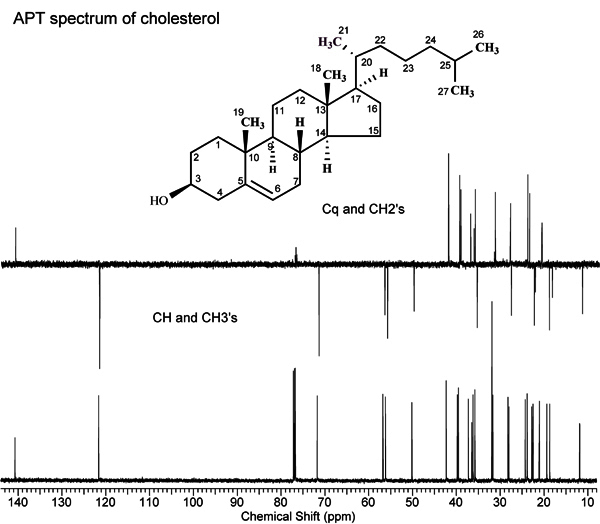
\includegraphics[keepaspectratio,width=4cm]{img/apt-spectra.jpg}}
\date{}

\begin{document}
\frame{\titlepage}

\section{Úvod}

\frame{
	\frametitle{}
	\begin{itemize}
		\item Cílem prezentace není výklad principů NMR, ale pouze pokrýt rozsah učiva probíraného na semináři C1605.
		\item Principy NMR můžete najít např. v prezentacích na následujících odkazech:
		\begin{itemize}
			\item \href{https://is.muni.cz/www/moravec/c5965_vybrane_analyticke_metody_v_chemii_konzervovani-restaurovani/}{C5965 Vybrané analytické metody v chemii konzervování-restaurování}
			\item \href{https://is.muni.cz/www/moravec/c7998_zaklady_experimentalni_nmr_spektroskopie/}{C7998 Základy experimentální NMR spektroskopie}
		\end{itemize}
	\end{itemize}
	\begin{center}
	\adjincludegraphics[width=0.5\textwidth]{img/nmr-scheme.jpg}
	\end{center}
}

\frame{
	\frametitle{}
	\begin{itemize}
		\item NMR studuje interakci atomových jader s radiofrekvenčním zářením v magnetickém poli.
		\item Aby bylo jádro NMR aktivní, musí mít nenulový jaderný spin.
		\item Jaderný spin získáme jako součet spinů nukleonů v jádře.
		\item Jádra s nulovým spinem, např. $^{12}$C, $^{16}$O, $^{32}$S jsou pro NMR nepoužitelná.
		\item Nejvhodnější jsou jádra se spinem $\frac{1}{2}$, např. $^{1}$H, $^{13}$C, $^{19}$F a $^{31}$P.
		\item Jádra s větším spinem lze také měřit, ale zpravidla poskytují výrazně širší signály, jde např. o $^{14}$N, $^{27}$Al nebo $^{35}$Cl.
	\end{itemize}
}

\section{Chemický posun a intenzita}
\frame{
	\frametitle{}
	\vfill
	\begin{itemize}
		\item Izolovaná jádra stejného izotopu budou v magnetickém poli rezonovat při stejné frekvenci.
		\item Pokud uvažujeme molekuly, je každé jádro ovlivněno také lokálními magnetickými poli, které jsou generovány vazebnými elektrony. Tím dochází ke změně rezonanční frekvence daného jádra.
		\item Změna je dána tzv. \textit{chemickým okolím} pozorovaného jádra a nazývá se \emph{chemický posun}. Označuje se $\delta$ a je dán vztahem:
	\end{itemize}
	\begin{center}
		$\delta = \frac{\nu - \nu_{TMS}}{\nu}$
	\end{center}
	\begin{itemize}
		\item $\nu_{TMS}$ je rezonanční frekvence standardu, $\nu$ je rezonanční frekvence signálu.
		\item Chemický posun je bezrozměrný, jelikož se jedná o velmi malé hodnoty, udává se v ppm.
		\item Chemický posun je, na rozdíl od rezonanční frekvence, nezávislý na hodnotě vnějšího magnetického pole.
	\end{itemize}
	\vfill
}

\frame{
	\frametitle{}
	\vfill
	\begin{itemize}
		\item Intenzita (přesněji integrální intenzita) je přímo úměrná zastoupení jader ve vzorku.
		\item Např. spektrum ethanolu (\ce{CH3-CH2-OH}) bude obsahovat tři signály v poměru intenzit 3:2:1.
		\item Na obrázku vidíme tři skupiny signálů, štěpení je způsobeno tzv. spin-spinovou interakcí, kterou ale v tomtu kurzu nebudeme řešit.
	\end{itemize}
	\begin{center}
		\adjincludegraphics[width=0.65\textwidth]{img/1H_NMR_Ethanol_Coupling_shown.png}
	\end{center}
	\vfill
}

\section{Počet signálů}
\frame{
	\frametitle{}
	\vfill
	\begin{itemize}
		\item Během NMR experimentu měříme signály zvoleného jádra.
		\item Počet signálů odpovídá počtu chemicky neekvivalentních jader ve studovaném vzorku.
		\item Pro $^1$H NMR spektrum ethanolu to tedy budou tři signály:
		\begin{itemize}
			\item \ce{CH3}
			\item \ce{CH2}
			\item \ce{OH}
		\end{itemize}
	\end{itemize}
	\begin{center}
		\adjincludegraphics[width=0.5\textwidth]{img/1H_NMR_Ethanol_Coupling_shown.png}
	\end{center}
	\vfill
}

\subsection{Butan}
\frame{
	\frametitle{}
	\vfill
	\begin{itemize}
		\item Chemicky neekvivalentní jsou jádra, jejichž chemické okolí se liší.
		\item To znamená, že uspořádání chemických vazeb a okolních atomů/skupin je různé.
		\item Pokud je možné jádra zaměnit některou z operací symetrie, jde o jádra chemicky ekvivalentní.
		\item Např. v molekule butanu máme dva typy vodíků: \ce{CH3} a \ce{CH2}.
		\item Vazbu mezi \ce{CH2} skupinami půlí zrcadlová rovina a dvojčetná rotační osa, díky kterým jsou obě \ce{CH3} a \ce{CH2} skupiny ekvivalentní.
		\item Butan tedy poskytne v $^1$H i $^{13}$C NMR dvojici signálů.
	\end{itemize}
	\begin{center}
		\adjincludegraphics[width=0.5\textwidth]{img/butane.png}
	\end{center}
	\vfill
}

\subsection{Diethylether}
\frame{
	\frametitle{}
	\vfill
	\begin{itemize}
		\item V případě diethyletheru je situace prakticky stejná.
		\item Molekula má zrcadlovou rovinu i rotační osu, která nám opět ztotožňuje \ce{CH3} a \ce{CH2} skupiny.
		\item Diethylether tedy poskytne v $^1$H i $^{13}$C NMR dvojici signálů.
		\item V případě $^1$H NMR bude poměr integrálních intenzit 6:4 neboli 3:2.
	\end{itemize}
	\begin{center}
		\adjincludegraphics[width=0.5\textwidth]{img/ethere.png}
	\end{center}
	\vfill
}

\subsection{Ethylester kyseliny octové}
\frame{
	\frametitle{}
	\vfill
	\begin{itemize}
		\item V případě ethylesteru kyseliny octové je situace odlišná.
		\item V molekule máme tři typy protonů: dvě \ce{CH3} skupiny a jednu \ce{CH2} a čtyři typy uhlíků, kromě dříve zmíněných ještě uhlík esterové skupiny.
		\item Jelikož molekula nemá žádnou operaci symetrie, která by skupiny ztotožňovala bude obsahovat $^1$H NMR spektrum tři signály a $^{13}$C NMR čtyři signály.
		\item Poměr intenzit signálů v $^1$H NMR spektru bude 3:2:3.
	\end{itemize}
	\begin{center}
		\adjincludegraphics[width=0.5\textwidth]{img/ethylacetate.png}
	\end{center}
	\vfill
}

\subsection{1,2,3-trifluorbenzen}
\frame{
	\frametitle{}
	\vfill
	\begin{itemize}
		\item Molekula má zrcadlovou rovinu, která zaměňuje červené fluory a vodíky v poloze meta.
		\item $^1$H NMR spektrum bude tedy obsahovat dva signály v poměru intenzit 2:1.
		\item $^{19}$F NMR spektrum bude obsahovat také dva signál v poměru intenzit 2:1.
		\item $^{13}$C NMR spektrum bude obsahovat čtyři signály, jeden od CF skupiny (černé), jeden od červených CF skupin, třetí od CH skupin v poloze meta a čtvrtý od CH skupiny v poloze para.
	\end{itemize}
	\begin{center}
		\adjincludegraphics[width=0.3\textwidth]{img/123-trifluorbenzen.png}
	\end{center}
	\vfill
}

\subsection{1-chlor-3,5-difluorbenzen}
\frame{
	\frametitle{}
	\vfill
	\begin{itemize}
		\item $^{1}$H NMR spektrum bude obsahovat dva signály v poměru 2:1, intenzivnější signál od protonů v \textit{ortho} poloze vůči chloru a druhý od protonu v \textit{para} poloze.
		\item $^{13}$C NMR spektrum bude obsahovat celkem čtyři signály, první od uhlíku nesoucího Cl atom, a další od uhlíků v polohách \textit{ortho}, \textit{meta} a \textit{para}.
		\item $^{19}$F NMR spektrum bude obsahovat jeden signál.
	\end{itemize}
	\begin{center}
		\adjincludegraphics[width=0.3\textwidth]{img/chlordifluorbenzene.png}
	\end{center}
	\vfill
}

\subsection{K procvičení}
\frame{
	\frametitle{}
	Vaše řešení mi můžete zaslat na mail ke kontrole -- hugo@chemi.muni.cz. Určete počet a intenzity signálů v $^{1}$H, $^{13}$C, $^{19}$F a $^{31}$P NMR spektrech.
	\begin{center}
		\adjincludegraphics[width=\textwidth]{img/examples.png}
	\end{center}
}

\end{document}